\chapter{Features}
\label{sec:Features}

\section{Features used to detect barcodes}
\label{sec:Features used to detect barcodes}
Several different features has been tried out but many of them have not given any satisfying result. Here are the features that have shown  best result.
\subsection{Standard deviation}
\label{sec:Standard deviation}
One good method to exclude tiles that don't contain any code is to compute the standard deviation of each tile. Tiles which contain code will have a high standard deviation; hence all data with standard deviation under a certain threshold can be discarded. This fast method to reduce the amount of data before applying other more complicated features. 

\subsection{Structure tensor}
\label{sec:Structure tensor}
The structure tensor is an effective way to detect 1D-codes and to distinguish between 1D- and 2D-codes. The structure tensor for a tile is produced by first computing the gradients, this can be done by convolving the tile with a sobel filter. The structure tensor is then calculated in the following way:
\begin{center}
\begin{math}
	T = \begin{pmatrix}
			(I_{x})^2 & I_{x}I_{y} \\ I_{x}I_{y} & (I_{y})^2
		\end{pmatrix}
\end{math}
\end{center}
The structure tensor can be used in several ways to estimate the structure inside the tile. Areas that contain 1D-codes will have a one dimensional structure, i.e. the gradient in this area will only vary in one direction. On the other hand, areas that contain 2D-codes the variation will be fairly equal in both directions. The amount of variation of the gradient is measured by studying the eigenvalues of the structure tensor. The following feature is calculated for each tile:
\begin{center}
\begin{math}
f = \frac{(\lambda_1 - \lambda_2)^2}{\lambda_1^2+\lambda_2^2}
\end{math}
\end{center}
This feature is a measure of how likely the tile contains 1D-codes.

\subsection{FAST corner detection}
\label{sec:FAST corner detection}
FAST (Features from Accelerated Segment Test) is described in \citep{Rosten:2006} and \citep{Rosten:2005}. This is a method to detect corners in images, which is a good way to distinguish between 1D- and 2D-codes. For a pixel \textit{p} with intensity \textit{I}, consider a circle of 16 pixel and a threshold \textit{t}. The pixel is considered to be a corner if there exist a set of n contiguous pixels in the circle which are all brighter than \textit{I+t} or darker than \textit{I-t}. The algorithm is described in \ref{FAST}.

\begin{figure}[H]
\centering
	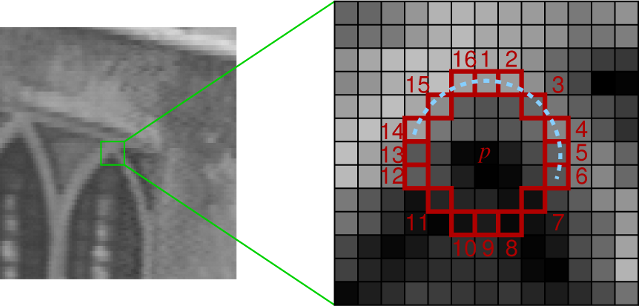
\includegraphics[scale=0.5]{FAST}
	\caption{Image describing FAST corner detection}
	\label{FAST}
\end{figure}

\subsection{Distance map}
\label{sec:Distance map}
A method for barcode detections using a distance map is described in \citep{Bodnar}. The objective of this method is to first calculate the edges in the image by using the canny edge detection algorithm. After that a distance transform is used which in each pixel calculates the closest distance to an edge. There after the mean and standard deviation for the distance map are calculated which are then used as features. The distance map has in this system been used only for detection of 1D-codes.
 
\subsection{Local binary pattern}
\label{sec:Local binary pattern}
Local binary pattern, which is described in \citep{Pietikainen:2010}, is a method that can be used for detection of 2D-codes. The basic idea is to compute a binary code for every pixel, based on the difference of the intensity between the pixel and the surrounding pixels, illustrated in \ref{LBP}. The binary code will then be transformed to a decimal scalar value. If a 3x3 neighbourhood is used there will be 256 different possible values. For each block a histogram will be calculated for all these values. Every bin in the histogram will then be used as a feature. If there is a bin for every possible value, there will be 256 features.

\begin{figure}[H]
\centering
	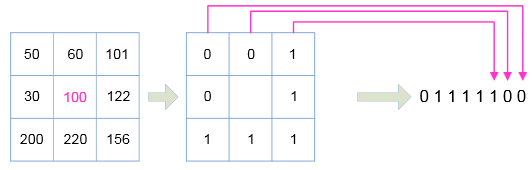
\includegraphics[scale=0.5]{LBP}
	\caption{Image describing local binary pattern}
	\label{LBP}
\end{figure}

\section{Features used for OCR}
\label{sec:Features used for OCR}
Here are the features that have been used for character detection.

\subsection{Two-rectangle features}
\label{sec:Two-rectangle features}
The two-rectangle features are based on the same idea as the Haar-features presented in \citep{Viola:2010}. This method was used in an earlier project regarding OCR at SICKIVP and showed a rather good result. For that reason it has been tried out in this project as well. The main concept is to use a large number of filters in different sizes consisting of two areas. The result from the filters will then be the difference of the sum of the pixel values between the two areas. There are 17 different filters illustrated in \ref{Two-rectangle} each in 64 different sizes. The sizes are in the range:
\begin{center}
	12x12, 12x16, 16x12, 16x16, 16x20, 20x16, 20x20......40x40
\end{center}
The filters can also have different positions which depends on the size of the tile that is used. For example if the tile has the size 120x120 a filter with the size 12x12 can have totally 100 positions without overlapping each other. For a tile with the size 120x120 there will in total be 28578 different features.  
\begin{figure}[H]
\centering
	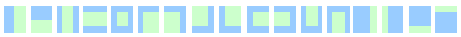
\includegraphics[scale=1]{rectfeatures}
	\caption{Image describing different types of two rectangle features}
	\label{Two-rectangle}
\end{figure}

To make the calculation of the rectangle features faster a s.k. integral image is used. This is a method presented in \citep{Viola:2010} for calculation of Haar-features. An integral image has the same size as the original image. The value for a pixel in the integral image is the sum of all the pixels above and to the left in the original image. If the $i(x,y)$ is the original image the integral image $ii(x,y)$ will be the following.

\begin{center}
	$ii(x,y) = \sum_{x' <= x, y' <= y} i(x',y')$
\end{center}

\subsection{Random point pairs features}
\label{sec:Random point pairs features}
One type of feature that has been tried out for OCR is a method presented in \citep{Nenad}. The idea is to compare a large amount of point pairs in a tile. The point pairs are randomly chosen but with some constraint. The first point in each pair is chosen from the central part of the tile and the the second point is chosen from the whole tile. There is also a constraint of the distance between the points in each pair. The reason for this is that the character should be somewhat centralized in the tile. If both points are at the edge of the image or if they are too close to each other there will likely be less information to gain. The same point pairs are used for every tile both during training and testing. For each tile the corresponding pixel values are compared in the following way:
 \begin{center}
\[ f_i = \left\{ 
   \begin{array}{l l l}
     1 & \quad I(p_1)<I(p_2)\\
     -1 & \quad I(p_1)>I(p_2)\\
     0 & \quad \text{otherwise}
   \end{array} \right.\]
 \end{center}
Each point pair will then correspond to a feature which can have one of three different values. 
\begin{figure}[H]
\centering
	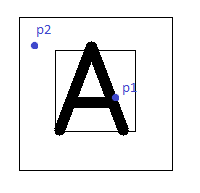
\includegraphics[scale=1]{PointPairs}
	\caption{Image describing two point pairs in a tile}
	\label{Two-rectangle}
\end{figure}



\subsection{Random line features}
\label{sec:Random line features}
The is a method similar to the random point pairs features. A large amount of point pairs are randomly chosen on the tile. Between the each point pair a line is defined.

\begin{figure}[H]
\centering
	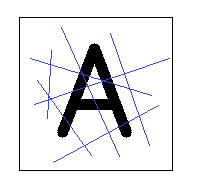
\includegraphics[scale=1]{RandomLines}
	\caption{Image describing some random lines in a tile}
	\label{Two-rectangle}
\end{figure}
  
% Local Variables:
% TeX-master: "main.tex"
% End:
